\documentclass[a4paper, 10pt]{article}
\usepackage[margin=0.5in]{geometry}

\usepackage{blindtext}
\usepackage{multicol}
\usepackage{booktabs}
\usepackage{amsmath}
\usepackage{mathtools}
\usepackage{float}
\usepackage{graphicx}
\usepackage{enumitem}
\usepackage{hyperref}
\usepackage{comment}

\graphicspath{{./outputs}}


\setlength{\columnsep}{1cm}
\title{ENPM 673: Perception for Autonomous Robots - Project 1}
\author{Aswath Muthuselvam \\ aswath@umd.edu}
\date{26th Feb 2022}

\begin{document}
	\maketitle
	\newlist{contract}{enumerate}{10}
	\setlist[contract]{label*=\arabic*.}
	\setlistdepth{10} 
	
	\begin{multicols}{2}
		
		\section{Question 1}
		\subsection{Separate coins}
		
		The coins are separated by lines of varying thicknesses, hence it can be removed by using a structuring element filled with zeros. I separated the coins using erosion.

		\subsection{Counting the coins}
		
		Now that the coins are separated, I used opencv findcontours() function to find all the 24 convex shapes. The number of detected contours are the number of coins present in the original image. Figure \ref{fig:op1} shows the complete process of erosion and contour detection.
				
		\begin{figure}[H]
			\centering
			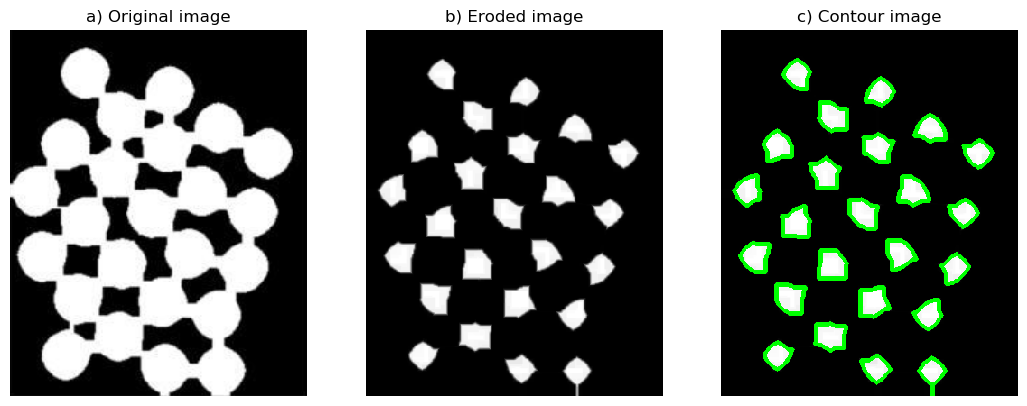
\includegraphics[width=\columnwidth]{/output1.png}
			\caption{AR Tag localization with FFT and Homography}
			\label{fig:op1}
		\end{figure}

		
		\begin{comment}
		
		\begin{figure*}
		\centering
		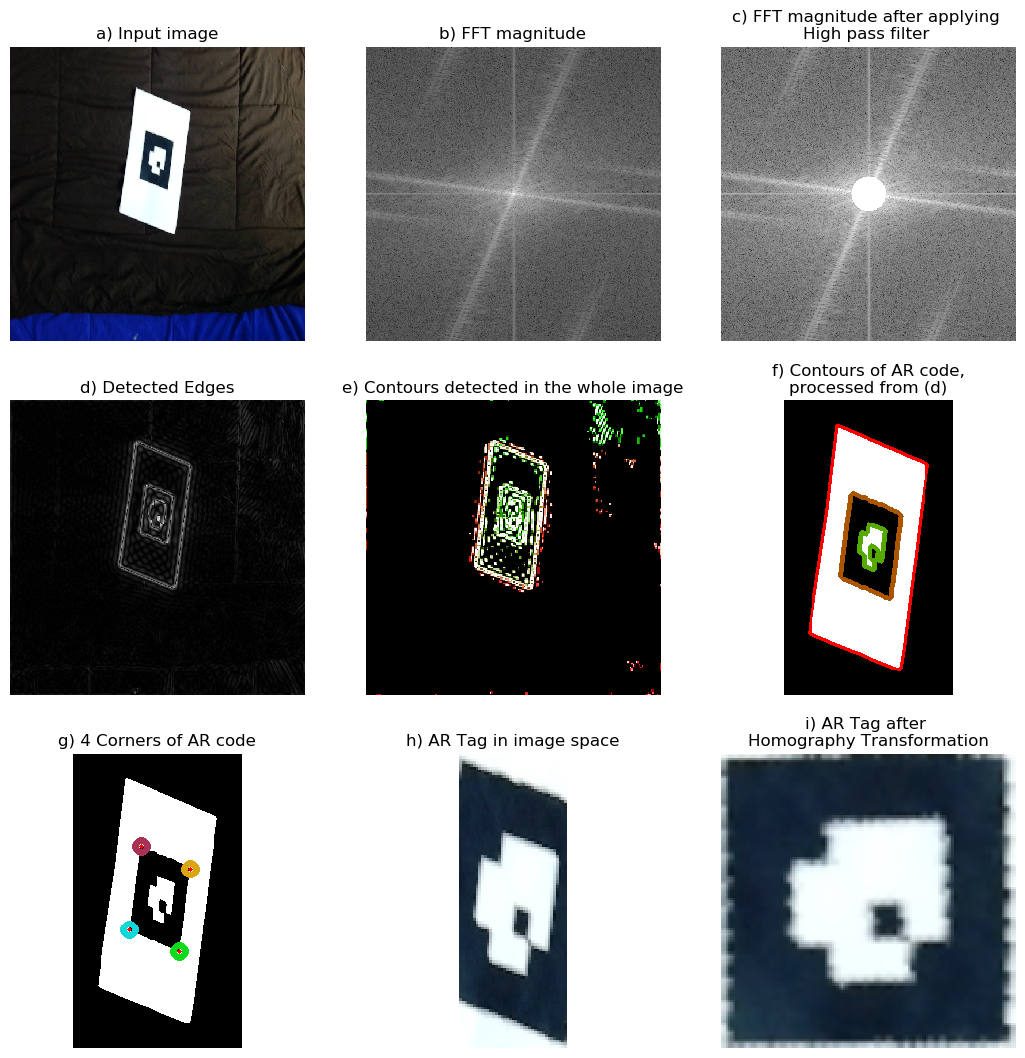
\includegraphics[width=0.75\textwidth]{/Q1/ARDetectionUsingFFt.png}
		\caption{Projecting the Testudo image on the ARTag}
		\label{fig:ARTa1g}
		\end{figure*}
		
		\end{comment}
		
		The homography transformation matrix is given by:
		\[
		\begin{bmatrix}
		x^{'} \\
		y^{'} \\
		w
		\end{bmatrix} =
		H\begin{bmatrix}
		x \\
		y \\
		1
		\end{bmatrix} = 
		\begin{bmatrix}
		h_{11} & h_{12} & h_{13}\\
		h_{21} & h_{22} & h_{23}\\
		h_{31} & h_{32} & h_{33}
		\end{bmatrix}
		\begin{bmatrix}
		x \\
		y \\
		1
		\end{bmatrix}
		\]
		
		\section{Problem 2}
		
	
		
		\begin{itemize}
		\item Firstly, the image is resized to the dimension of 200 x 200 to match the world coordinates.
		\item A “changeOrient” is defined to reorient the tag. The image, according to the orientation of the tag is rotated by using this function.
		\item After transformations and inverse homography, the tag in the image is warped to form a black background
		\item The function cv2.bitwise\_or is used to superimpose the testudo image on the AR tag.
		\end{itemize}
	

		
		\subsection{}		
		
		The steps to compute projection matrix is given as follows:
		\begin{itemize}
			\item Define h1,h2,h3 as the 3 columns in the homography
			matix H
			\item Compute scale factor $\lambda = \Big[ \dfrac{(K^{-1}h1 + K^{-1}h2)}{2}\Big]^{-1}$
			\item $\tilde{B} = \lambda K^{-1}H$ 
			\item $B = \tilde{B}(-1)^{|\tilde{B}|<0}$ i.e. $B = -\tilde{B}$ if B is negative, else $B = \tilde{B}$. b1,b2,b3 are defined as column vectors of B.
		\end{itemize}
		

		
	\end{multicols}
	
\end{document}
